\chapter{Quadratic Functions}
\label{ch:quadfunc}

\chapquote{Nature creates curved lines while humans create straight lines.}{Hideki Yukawa\\Japanese theoretical physicist}

In the last few chapters, we have studied quadratic equations, the methods for solving them, and the various algebraic rules for manipulating the kinds of answers we get (square roots). We turn now to quadratic relationships and situations that can be represented using quadratic functions. We'll look more closely at the equations and graphs of quadratic functions, and look closely at one of the classic applications from physics.

% % % % % % % % % % % % % % % % % % % % % % % % % % % % % % % % % % % % % % % % 
\section{Quadratic Relationships}
\label{sec:quadrelationships}

%\begin{boxedexplore}[Extended Exploration: Staking a Claim]
%LINK
%\end{boxedexplore}
\addtodoitem{Link to extended exploration: Staking a claim}

\begin{boxedexplore}[Compost Heap]
Uncle Fran\c{c}ois wants to make a compost heap in the corner of his vegetable garden. He plans to enclose a rectangular area using the two existing walls of the garden, plus 8 yards of leftover fencing.

\begin{center}
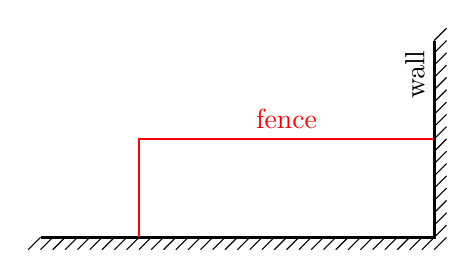
\begin{tikzpicture}[scale=0.625]
	\draw[very thick] (0,0) -- (8,0) -- (8,4);
	\draw(8,4) node[rotate = 90, above left]{wall}; 
	\foreach \x in {0, 0.25,...,8.25} \draw (\x,0) -- (\x-0.25, -0.25);
	\foreach \y in {0, 0.25,...,4} \draw (8,\y) -- (8.25, \y+0.25);
	\draw[red, thick] (2,0) -- (2,2) -- node[above]{fence} (8,2);
\end{tikzpicture}
\end{center}

If he wants to enclose the largest possible area, how should he arrange the fence? What is the maximum area he can enclose?
\end{boxedexplore}

A good way to start this problem might be simply to get our hands dirty and see what happens.\footnote{After all, we are talking about a compost heap.} If Fran\c{c}ois has 8 yards of fencing, he could fence in a rectangle that is, say, 2 meters long and 6 meters wide. That would give him a compost heap with an area of 12 square yards. Can he enclose more area than this?

To enumerate all of Fran\c{c}ois's options, suppose we set up a data table that shows the dimensions of the rectangle and its area.

\begin{table}
\begin{tabular}{C{2cm}C{2cm}|C{2.5cm}}
\text{Length (yd)} & \text{Width (yd)} & \text{Area (sq. yd)}\\\hline
0 & 8 & 0\\
1 & 7 & 7\\
2 & 6 & 12\\
3 & 5 & 15\\
4 & 4 & 16\\
5 & 3 & 15\\
6 & 2 & 12\\
7 & 1 & 7\\
8 & 0 & 0
\end{tabular}
\end{table}

Aha! There are some patterns to be found here. It certainly seems that the 4-by-4 rectangle (the square, that is) encloses the most area. Indeed, if we plot a graph of length versus area, we have another representation of this maximum value.

\begin{figure}
\resizeplot{0}{0}{8}{16}
\begin{tikzpicture}
	\begin{axis}[standard, labeloutsideaxis, xlabel={Rectangle length (yd)}, ylabel={Rectangle area (sq. yd)}]
		\addplot[algcurve, blue, domain=-0:8]{x*(8-x)};
		\addplot[algpoints, blue] coordinates{(0,0)(1,7)(2,12)(3,15)(4,16)(5,15)(6,12)(7,7)(8,0)};
	\end{axis}
\end{tikzpicture}
\end{figure}

Note that we connected the dots in our graph. Under the given constrains, a reasonable length for the rectangle is any real numbers between 0 and 8. Of course, if the length is 0, then it's not really a rectangle\ldots so we should exclude the value $x=0$ as an option. The same goes for $x=8$ (since in this case the width of the rectangle is zero). So, this is the domain of our quadratic function in the context of the problem: $x$ must be greater than zero and less than 8, or $0<x<8$.

Note that the range of our function includes all $y$ values between 0 and 16 square yards. In fact given the domain, we have $0 < y \leq 16$, since the area can be 16, but can never actually be 0.

This graph demonstrates a number of important properties about quadratic functions: We get a smooth U-shaped graph that is perfectly symmetrical, and which has an extreme value (a maximum value in this case).\footnote{There is an interesting geometric definition of a parabola. First note that a circle is the set of all points that are a fixed distance from a given point. The ``given point'' is called the center of the circle, and the ``fixed distance'' is called the radius of the circle. A parabola is the set of all points which are the same distance from a fixed point (called the \textit{focus}) and a fixed line (called the \textit{directrix}). We'll see more definitions like this later, when we study the so-called \textit{conic sections} in Algebra 2.} These aspects of the graph all have names.

\begin{boxeddef}[Parabola]
The U-shaped graph of a quadratic function.
\end{boxeddef}

\begin{boxeddef}[Vertex]
The extreme (lowest or highest) point on a parabola.
\end{boxeddef}

\begin{boxeddef}[Axis of symmetry]
The imaginary line that passes through the vertex and divides the parabola into two symmetric halves.
\end{boxeddef}

We also see a familiar pattern in the sequence of area values: a constant second difference.

\begin{table}
\begin{tabular}{r|*{9}{C{0.75cm}}}
Area values			& 0 & 7 & 12 & 15 & 16 & 15 & 12 & 7 & 0\\
Differences			& ~ & 7 & 5 & 3 & 1 & -1 & -3 & -5 & -7\\
Second differences	& ~ & ~ & -2 & -2 & -2 & -2 & -2 & -2 & -2\\
\end{tabular}
\end{table}

Recall that we can't simply rely on the ``increases then decreases'' pattern (or the reverse) to determine whether a sequence or a data table is quadratic. We must look closely at the pattern an find that constant second difference.

%Also interesting is that the second difference is negative. Does that have anything to do with the In general, the sign of the second difference will tell if the parabola is going to increase then decrease (sad parabola = negative 2nd difference) or if it is going to decrease then increase (happy parabola = positive 2nd difference)

\subsection{A rectangular rule}

What equation describes our rectangle area function? In our graph we are displaying area as a function of length. We know how to calculate the area of a rectangle: that's length times width. The trick in this case is to notice that the length ($\ell$) and width ($w$) of the rectangle always add up to 8 (the fixed length of fence we have to work with). So:
\[\ell + w = 8 \qquad\text{or}\qquad \ell = 8-w\]

So, we can write a rule for $A(\ell)$, the area of the rectangle as a function of its length: $A(\ell) = \ell(8-\ell)$. Of course we can always use the distributive property to eliminate those parentheses:
\[A(\ell) = \ell(8-\ell) = 8\ell - \ell^2\]
So, we have two different forms of our quadratic equation! In fact, there is a third form that is also important. In the next section (and then again in the next chapter), we will look more closely at quadratic rules. In the meantime, note that we did something a bit like we did we linear functions. Back in \cref{ch:linear}, we turned point-slope form into slope-intercept form using the distributive propoerty and combining like terms. Part of our goal now will be to understand the techniques that allow us to convert between the different forms of a quadratic equation.


\subsection{Powerful symmetry}

The symmetrical qualities of a quadratic function will be very helpful to us. We have already seen how the symmetry of the square can help us to solve quadratic equations (via the quadrangle method), and we will use the symmetry of the parabola, too.

\begin{figure}
\resizeplot{-1}{-4}{9}{17}
\begin{tikzpicture}
	\begin{axis}[standard]
		\addplot[algcurve, blue, domain=-0.5:8.5]{x*(8-x)};
		\addplot[algpoints, blue] coordinates{(0,0)(1,7)(2,12)(3,15)(4,16)(5,15)(6,12)(7,7)(8,0)};
		\draw[<->, red, dashed, thick] (axis cs: 4,-5) -- (axis cs: 4, 18);
	\end{axis}
\end{tikzpicture}
\end{figure}

Note that the line of symmetry, the line $x=4$ in this case, cuts the parabola into two identical halves. This graph has two $x$-intercepts that are equidistant from
the line of symmetry. In fact, every point (other than the vertex) has a buddy on the other side of the line of symmetry: a point that is at the same $y$-value, and an equal distance form the line of symmetry.

\subsubsection{Speaking of intercepts}

Every quadratic function has one and only one $y$-intercept. The situation is slightly more complicated for $x$-intercepts. The graph above has two $x$-intercepts. Can you picture the other possibilities?

\begin{figure}
\begin{minipage}{0.32\textwidth}
	\centering
	\begin{tikzpicture}
	\begin{axis}[standard, fullsize]
		\addplot[algcurve, red, domain=0:6]{(x-3)^2+1};
		\addplot[algcurve, red, domain=-8.25:4.25]{-0.2*(x+2)^2-2};
	\end{axis}
	\end{tikzpicture}
	Parabolas with 0 $x$-intercepts.
\end{minipage}
%
\begin{minipage}{0.32\textwidth}
	\centering
	\begin{tikzpicture}
	\begin{axis}[standard, fullsize]
		\addplot[algcurve, green!50!black, domain=-0.2:6.2]{(x-3)^2};
		\addplot[algcurve, green!50!black, domain=-9:5]{-0.2*(x+2)^2};
	\end{axis}
	\end{tikzpicture}
	Parabolas with 1 $x$-intercept.
\end{minipage}
%
\begin{minipage}{0.32\textwidth}
	\centering
	\begin{tikzpicture}
	\begin{axis}[standard, fullsize]
		\addplot[algcurve, violet, domain=-0.35:6.35]{(x-3)^2-1};
		\addplot[algcurve, violet, domain=-9.75:5.75]{-0.2*(x+2)^2+2};
	\end{axis}
	\end{tikzpicture}
	Parabolas with 2 $x$-intercepts.
\end{minipage}
\end{figure}

A parabola may have 0, 1, or 2 $x$-intercepts. If there are no $x$-intercepts, then the graph lies entirely above or below the $x$-axis. If there is only one $x$-intercept, then it must be the vertex! Otherwise every point comes with a buddy at the same height.


\subsubsection{A final thought on fixed perimeters}

You may have noticed that the rectangle which maximized the area of the compost heap was, in fact, a square. This is true in general: given a fixed perimeter, many rectangles can be draw which have that perimeter, and the one with the largest area will be the square.

What if we lift the restriction that the shape be a rectangle? Given a fixed perimeter, could we create a hexagon with area larger than our square? What shape should we make to get the maxmum possible area of all possible shapes?


% % % % % % % % % % % % % % % % % % % % % % % % % % % % % % % % % % % % % % % % 
\section{Vertex form of a quadratic function}
\label{sec:vertexform}

\begin{boxedexplore}[Move that curve]
The graph below shows the parent of the quadratic family, $y=x^2$, and a offspring function that has the same shape but is shifted so that the vertex is at the point $(3, 4)$.

\begin{center}
	\resizeplot{-4}{-4}{10}{16}
	\begin{tikzpicture}
	\begin{axis}[standard]
		\addplot[algcurve, blue, domain=-4:4]{x^2};
		\addplot[algcurve, red, domain=-0.5:6.5]{(x-3)^2+4};
		\addplot[algpoints,blue] coordinates{(0,0)};
		\addplot[algpoints,red] coordinates{(3,4)};
		\node[below right, red] at (axis cs: 3,4) {$(3,4)$};
	\end{axis}
	\end{tikzpicture}
\end{center}

Look back over our discussion of transformations (back in \cref{sec:threefamilies}), and write an equation for the offspring graph. Tinkering around with some some \href{https://www.desmos.com/}{graphing technology} may be helpful!
\end{boxedexplore}

With some careful observation and a bit of tinkering, we can move the parent parabola to its new position using the rule:
\[y-4=(x-3)^2 \qquad\text{or}\qquad y = (x-3)^2+4\]
The ``$y-4$'' in the rule controls the up-and-down movement of the parabola, shifting it 4 units upwards in this case. The ``$x-3$'' inside the parentheses is the component that controls left-and-right movement. The values 3 and 4 are related to the location of the vertex of the parabola. Naturally enough, an equation like this is called the \gls{vertex form}.

\begin{boxeddef}[Vertex form of a quadratic function]
An equation of the form \[y = a(x-h)^2 + k,\] where $a\neq0$, is a quadratic function in vertex form. The point $(h,k)$ is the vertex of the parabola.
\end{boxeddef}

Note the similarity of this form to the point-slope form of a line:
\[\begin{array}{rl}
\text{point-slope form of a linear function: } & y = m(x-x_1) + y_1\\
\text{vertex form of a quadratic function: } & y = a(x-h)^2 + k
\end{array}\]


\subsection{Graphing quadratics in vertex form}

To graph a quadratic function give its rule, we could make a table of values that has many points. In the past, we've plotted 7 data points to make a graph: for example using the integers between $-3$ and 3 as the $x$-values.

When working with linear equations, though, we learned that we need just two points to graph a line. This cuts down on the work! There's good news here, too: every parabola can be created with exactly 3 points. Our goal as we graph is to find a few strategic points to plot so that we can sketch a reasonable curve efficiently.

Good candidates for ``strategic points'' include: the vertex, the $y$-intercept, and the $x$-intercepts (if they exist). We will also take advantage of the fact that parabolas are symmetric.

If we are given a line in vertex form, then the location of the vertex (and the line of
symmetry) is right there in the equation. That's a huge benefit of vertex form!

For example, given the function $y= \frac{2}{3}(x-3)^2+2$, we can read the location of the vertex directly from the rule: $(3, 2)$. This also tells us that the line of symmetry (which passes through the vertex) must be the vertical line $x=3$.

What else can we learn? The coefficient 3 in front tells us that this parabola will open upwards (since 3 is positive), and that it will be narrower than $y=x^2$ (the parent function for this family).

Plus, since the parabola opens upwards and has its vertex above the $x$-axis, this parabola must be one of those that has no $x$-intercepts. We really can learn a lot just from looking at the equation!

We still have only one point, though, and we need three points to plot our graph. How can we find the $y$-intercept? This is the value of the function when $x=0$, so we can evaluate the function at that point and see what we get!
\begin{commwork}
y & \tfrac{2}{3}(x-3)^2+2
& original function
\\
y & \tfrac{2}{3}(0-3)^2+2
& let $x=0$ to find the $y$-intercept
\\
& \tfrac{2}{3}(-3)^2+2
\\
& \tfrac{2}{3}(9)+2
\\
& 6+2
\\
& 8
\end{commwork}

So, the $y$-intercept is the point $(0,8)$. We now have two points that we can plot on our graph. How do we find the third?

\begin{figure}
	\resizeplot{-1}{-1}{9}{9}
	\begin{tikzpicture}
	\begin{axis}[standard]
%		\addplot[algcurve, blue, domain=-0.25:6.25]{(2/3)*(x-3)^2+2};
		\addplot[algpoints,blue] coordinates{(3,2)(0,8)};
		\draw[<->,dashed,thick] (axis cs: 3,-1) -- (axis cs: 3,9);
	\end{axis}
	\end{tikzpicture}
\end{figure}

Here's where the symmetry of the parabola comes in handy. The point that is symmetrical to the $y$-intercept will be the same horizontal distance from the line of symmetry, and at the same height as the $y$-intercept. So, the point we want is $(6, 8)$ -- it is at the same height (8 units), and three units away, but on the other side of the line of symmetry. We can plot this point, and graph the parabola!

\begin{figure}
	\resizeplot{-1}{-1}{9}{9}
	\begin{tikzpicture}
	\begin{axis}[standard]
		\addplot[algcurve, blue, domain=-0.25:6.25]{(2/3)*(x-3)^2+2};
		\addplot[algpoints,blue] coordinates{(3,2)(0,8)(6,8)};
		\draw[<->,dashed,thick] (axis cs: 3,-1) -- (axis cs: 3,9);
	\end{axis}
	\end{tikzpicture}
\end{figure}

Now, if we find that the vertex lies on the $y$-axis, then we can't use the $y$-intercept as our second point (because the vertex \textit{is} the $y$-intercept). We'll address graphing parabolas like this in the next section.


% % % % % % % % % % % % % % % % % % % % % % % % % % % % % % % % % % % % % % % % 
\section{Standard form of a quadratic function}
\label{sec:standardformquad}

\begin{boxedexplore}[Rename that curve]
In the last section, we wrote a rule for shifting the parent of the quadratic family, $y=x^2$, such that the vertex was at the point $(3, 4)$.

\begin{center}
	\resizeplot{-4}{-4}{10}{16}
	\begin{tikzpicture}
	\begin{axis}[standard]
		\addplot[algcurve, blue, domain=-4:4]{x^2};
		\addplot[algcurve, red, domain=-0.5:6.5]{(x-3)^2+4};
		\addplot[algpoints,blue] coordinates{(0,0)};
		\addplot[algpoints,red] coordinates{(3,4)};
		\node[below right, red] at (axis cs: 3,4) {$(3,4)$};
	\end{axis}
	\end{tikzpicture}
\end{center}

The rule we wrote was $y=(x-3)^2 + 4$. Use everything you know about simplifying algebraic expressions to rewrite this rule in its simpliest form. Use \href{https://www.desmos.com/}{graphing technology} to verify that your simplified rule and the original rule produce the same graph.
\end{boxedexplore}

The first problem with the rule in the startup exlploration is that patenthesized expression. To eliminate this, we can use the distributive property (raising a sum to a power). After that, we'll need to combine some like terms:
\begin{commwork}
y & (x-3)^2 + 4
& the original equation
\\
& (x-3)(x-3) + 4
& expand the exponent
\\
& x(x-3) - 3(x-3) + 4
& distribute one $(x-3)$ over the other
\\
& x^2 - 3x - 3x + 9 + 4
& distribute again (watch the signs!)
\\
& x^2 - 6x + 13
& combine like terms
\end{commwork}
Now we have a new equation that is equivalent to the original: an equation in what we call \textit{standard form}.

\begin{boxeddef}[Standard form of a quadratic function]
An equation of the form \[y = ax^2 + bx + c,\] where $a \neq 0$, is a quadratic function in standard form.
\end{boxeddef}

In some sense, this equation has obscured key things about the parabola. It is not obvious, for instance, where the vertex is. But, something new has been revealed. What does that ``$+13$'' tell us about the graph?

Compare this form to the slope-intercept form of a line:
\[\begin{array}{rl}
\text{slope-intercept form of a linear function: } & y = mx + b\\
\text{standard form of a quadratic function: } & y = ax^2 +bx+ c
\end{array}\]
Note that the constant term in each case is the $y$-intercept of the graph. This makes sense, for if we evaluate each function at $x=0$ (that's the $y$-axis), then any term with an $x$ in it disappears and we are left only with the constant term. To be clear in the case of our standard-form quadratic: when $x=0$, we have
\[y = a\cdot0^2 + b\cdot0 + c = 0 + 0 + c = c.\]


\subsection{Graphing standard form}

Vertex form is nice for graphing, since the vertex is right there in the equation. When taksed with graphing an equation in standard form, our strategy will be much the same\ldots\ though we'll have to do a bit more work. Our first goal will be to find the vertex.

\subsubsection{Axis of symmetry}

As with all things parabolic, symmetry is our friend. We know that the point $(0,c)$ is on the parabola: that's the $y$-intercept. If we assume that this point is not the vertex of the parabola, then we know there is a second point on the parabola, also at height $c$. What is the $x$-coordinate of this other point?

We can figure that out by solving an equation. We want to know what $x$ values lead to $y=c$, so that is like solving the equation:
\[ax^2 + bx + c = c \qquad\text{or, by SPOE}\qquad ax^2 + bx = 0\]

We will soon learn a quick way to solve this equation, but in the meantime, we can use the quadrangle method! We multiply through by $a$ (to make the quadratic term a perfect square) and then by 4 (to ensure that the linear term has an even coefficient). This gives us:
\[4a^2x^2 + 4abx = 0\]

Arranging in the quadrangle gives us:
\quadrangle{2ax}{b}{4a^2x^2}{2abx}{\color{red}b^2}

We must add $b^2$ to both sides of our equation, to accomodate the quadrangle diagram. From here, it's clear sailing:
\begin{commwork}
4a^2x^2 + 4abx & 0
&\\
4a^2x^2 + 4abx + b^2 & b^2
& APOE
\\
(2ax+b)^2 & b^2
& based on the quadrangle method
\\
2ax+b & b \OR -b
& square root of both sides
\\
2ax & 0 \OR -2b
& SPOE
\\
x & 0 \OR \tfrac{-b}{a}
\end{commwork}

So, we have discovered two $x$-values for which the quadratic equation produces $y=c$. Those values are $x=0$ (we knew this one already, but it's nice that our work confirms our expectations!), and $x = \frac{-b}{a}$. What does this tell us?

\begin{figure}
\resizeplot{-2}{-2}{6}{8}
\begin{tikzpicture}
	\begin{axis}[
		clip=false,
		axis lines = middle,
		axis line style={thick, <->, shorten >=-8pt, shorten <=-8pt},
%		every axis/.append style={font=\footnotesize},
		xlabel={$x$},
		ylabel={$y$},
		xtick={4},
		xticklabels={$\dfrac{-b}{a}$},
		ytick={5},
		yticklabels={$c$},
%		grid = both,
%		grid style={gray!25},
		xmin=\mminx,		% start the diagram at this x-coordinate
		xmax=\mmaxx,	% end the diagram at this x-coordinate
		ymin=\mminy,		% start the diagram at this y-coordinate
		ymax=\mmaxy,		% end the diagram at this y-coordinate
		]
		\addplot[algcurve, blue, domain=-0.75:4.75]{(x-2)^2+1};
		\addplot[algpoints, blue] coordinates{(0,5)(4,5)};
		\draw[<->, red, dashed, thick] (axis cs: 2,-2) -- (axis cs: 2, 8);
		\draw[dashed, thick] (axis cs: 4,0) -- (axis cs: 4, 5);
	\end{axis}
\end{tikzpicture}
\end{figure}

We know that the line of symmetry must be exactly halfway between these two points. In other words, exactly halfway between 0 and $\frac{-b}{a}$. We just have to divide that distance in half and we have found an equation for the line of symmetry!

\begin{boxeddef}[Axis of symmetry]
Given a quadratic equation of the form $y=ax^2+bx+c$, the axis of symmetry for the parabola is the vertical line at \[x=\frac{-b}{2a}.\]
\end{boxeddef}

Once we have found the axis of symmetry, we know the $x$-coordinate of the vertex. We can then evaluate the function at this point to find the $y$-coordinate.

\begin{boxedex}
Locate the vertex of the parabola given by $y=2x^2+12x+11$.

\exsoln\ We can use our equation for the line of symmetry to start us out. In this case, we have $a=2$ and $b=12$, the this parabola is symmetric about the line
\[x = \frac{-b}{2a} = \frac{-12}{2\cdot2} = \frac{-12}{4} = -3.\]
So the $x$-coordinate of the vertex is $-3$. We plug this value into our equation to determine the correspondig $y$-coordinate:
\begin{commwork}
y & 2x^2 + 12x + 11
\\
& 2(-3)^2 + 12(-3) + 11
\\
& 18 - 36 + 11
\\
& -7
\end{commwork}
So, we have located the vertex! It is the point $(-3, -7)$.
\end{boxedex}

Once we have found the vertex, we have one point on our parabola. To graph it, we must find two more. If the vertex is not on the $y$-axis, then this job isn't too hard because we get a second point for free: the $y$-intercept!

Once we plot the vertex and the $y$-intercept, we can find and plot the point that is symmertical to the $y$-intercept on the othet side of the axis of symmetry.

\begin{boxedex}
Graph the parabola given by $y=2x^2+12x+11$.

\exsoln\ In the previous example, we found the vertex of this parabola to be $(-3,-7)$. We can also see from the equation that the $y$-intercept is $(0,11)$. We can plot these points quite easily:

\resizeplot{-10}{-10}{5}{15}
\begin{center}
	\begin{tikzpicture}
	\begin{axis}[standard]
%		\addplot[algcurve, violet, domain=-6.25:0.25]{2*(x+3)^2-7};
		\addplot[algpoints,violet] coordinates{(0,11)(-3,-7)}; %(-6,11)};
		\draw[<->,dashed,thick] (axis cs: -3, -10) -- (axis cs: -3, 15);
	\end{axis}
	\end{tikzpicture}
\end{center}

Now, we're on the hunt for the point that is symmetrical to the $y$-intercept. This point will be at the same height ($y=11$) but on the other side of the line of symmetry. The line of symmetry is three units from the $y$-axis, so the point we seek must be three units away on the other side of the line of symmetry. That means we want the point $(-6, 11)$. We can plot this point, and graph the parabola!

\begin{center}
	\begin{tikzpicture}
	\begin{axis}[standard]
		\addplot[algcurve, violet, domain=-6.25:0.25]{2*(x+3)^2-7};
		\addplot[algpoints,violet] coordinates{(0,11)(-3,-7)(-6,11)};
		\draw[<->,dashed,thick] (axis cs: -3, -10) -- (axis cs: -3, 15);
	\end{axis}
	\end{tikzpicture}
\end{center}
\end{boxedex}

As we mentioned above, we may find that the vertex of our parabola lies on the $y$-axis. In this case we can't use the $y$-intercept as our second point (because the vertex and the $y$-intercept are \textit{the same point}). So in this case, we are forced to choose another $x$-value and compute it's corresponding $y$-value. Since we have the luxury of choosing our $x$-value it makes sense to try and choose a value that makes our calcualtions easy, but that's up to us to decide.

Can we predict what the equation of such a quadratic will look like? If the axis of symmetry is the vertical line $x=0$, then the $x$-coordinate of the vertex is 0. So in vertex form, $h=0$. This means that we have:
\[y=a(x-h)^2+k = a(x-0)^2+k = ax^2+k\]
So, if the quadratic function has no linear term (no $bx$ term), then it's line of symmetry is $y$-axis.

\begin{boxedex}
Graph the parabola $f(x)=-\frac{1}{4}x^2 + 9$.

\exsoln\ This quadratic has no linear term, the line of symmetry is the $y$-axis. The $y$-intercept is 9, and the coefficient $a$ is negative, so the parabola opens downward. But now it's up to us to find another two points.

Suppose we choose $x=4$, which might help to eliminate that fraction. In that case, we have:
\[f(4) = -\frac{1}{4}(4)^2 + 9 = -\frac{1}{4}(16)+9 = -4+9 = 5.\]
So the point $(4,5)$ is on the graph. Because of symmetry, this means that the point $(-4,5)$ is also on the graph. We have our three points!

\resizeplot{-10}{-10}{10}{10}
\begin{center}
	\begin{tikzpicture}
	\begin{axis}[standard]
		\addplot[algcurve, green!50!black, domain=-8:8]{-0.25*x^2+9};
		\addplot[algpoints,green!50!black] coordinates{(0,9)(-4,5)(4,5)};
	\end{axis}
	\end{tikzpicture}
\end{center}
\end{boxedex}

In the previous example, we have another option: we could find the $x$-intercepts, which occur when $y=0$. Here's how we'd do it for the example:
\begin{commwork}
y & -\frac{1}{4}x^2 + 9
& original equation
\\[1ex]
0 & -\frac{1}{4}x^2+9
& let $y=0$ to find the $x$-intercepts
\\[1ex]
-9 & -\frac{1}{4}x^2
& SPOE
\\[1ex]
36 & x^2
& MPOE
\end{commwork}
This means that $x$ must be 6 or $-6$. In other words, the $x$-intercepts are the points $(6,0)$ and $(-6,0)$, and this conclusion is shown on the graph that we drew above!

Although the numbers worked out nicely in this case, finding $x$-intercepts can require some clever thinking, and some new algebraic tools. It will be a topic we investigate more closely in \cref{ch:factoring}.


\subsection{Standard to vertex form: Completing the square}

Converting from vertex form to standard form is easy: we simply expand the squared expression using the distributive property, and then combine like terms. Converting in the other direction is harder, although we have already seen a technique that is helpful: the quadrangle method.

Note that an equation in vertex form has a square inside it: the $(x-h)^2$ term is a square with sides of length $(x-h)$. Can we manipulate a standard-form quadratic to find a hidden square?

Let's take a specific example: consider the equation $y=x^2+8x+11$. Does this expression make a square? One way to visualize this is to imagine our trusty algebra tiles. The given quadratic expression in this case can be represented by the algebra tiles:

\begin{figure}
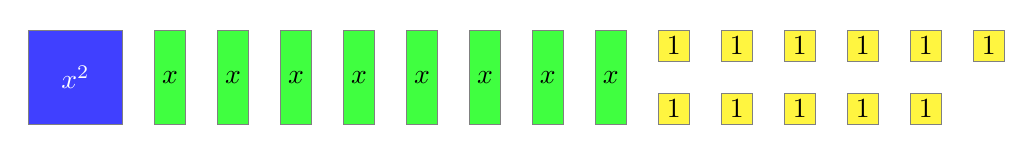
\begin{tikzpicture}[scale=0.4]
	\draw[gray, fill=blue!75] (0,0) rectangle node[white]{$x^2$} (3,3);
	\foreach \x in {4, 6, ..., 18} {
		\draw[gray, fill=green!75] (\x,0) rectangle node[black]{$x$} (\x+1, 3);
	}
	\foreach \x in {20, 22, ..., 28} {
		\draw[gray, fill=yellow!75] (\x,0) rectangle node[black]{$1$} (\x+1, 1);
		\draw[gray, fill=yellow!75] (\x,2) rectangle node[black]{$1$} (\x+1, 3);
	}
	\draw[gray, fill=yellow!75] (30,2) rectangle node[black]{$1$} (31, 3);
\end{tikzpicture}
\end{figure}

If we try to arrange these tiles into a square, we're a few tiles short. What do we need to \textit{complete the square}?

\begin{figure}
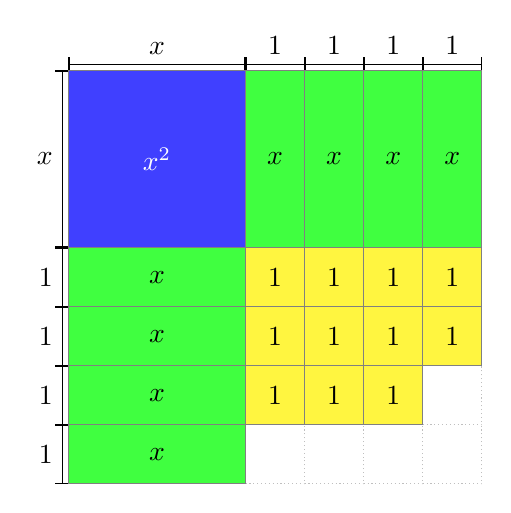
\begin{tikzpicture}[scale=0.75]
	\draw[|-|] (0,0.1) -- node[above]{$x$} (3,0.1);
	\draw[|-|] (-0.1,0) -- node[left]{$x$} (-0.1,-3);
	\draw[gray, fill=blue!75] (0,0) rectangle node[white]{$x^2$} (3,-3);
	\foreach \x in {3,...,6} {
		\draw[|-|] (\x,0.1) -- node[above]{1} (\x+1,0.1);
		\draw[gray, fill=green!75] (\x,0) rectangle node[black]{$x$} (\x+1,-3);
	}
	\foreach \y in {-3,...,-6} {
		\draw[|-|] (-0.1,\y) -- node[left]{1} (-0.1,\y-1);
		\draw[gray, fill=green!75] (0,\y) rectangle node[black]{$x$} (3,\y-1);
	}
	% two rows of yellow tiles
	\foreach \x in {3,...,6} {
		\foreach \y in {-3,...,-4}
			\draw[gray, fill=yellow!75] (\x, \y) rectangle node[black]{1} (\x+1,\y-1);
	}
	% plus three stray yellow tiles
	\foreach \x in {3,...,5} \draw[gray, fill=yellow!75] (\x, -5) rectangle node[black]{1} (\x+1, -6);
	% plus the remaining phantom tiles
	\draw[gray!50, densely dotted] (6, -6) -- (7,-6) -- (7, -5);
	\foreach \x in {3,...,6} \draw[gray!50, densely dotted] (\x, -7) -- (\x+1,-7) -- (\x+1, -6);
\end{tikzpicture}
\end{figure}

If only we had 5 more 1-unit tiles in our diagram! Well, we can accomplish this by changing our original equation using the POEs, just like we did in the quadrangle method:
\begin{commwork}
y & x^2 + 8x + 11
& original equation
\\
y+5 & x^2 + 8x + 16
& APOE: add 5 to both sides
\\
y+5 & (x+4)^2
& based on the quadrangle diagram
\\
y & (x+4)^2 - 5
& SPOE, to isolate $y$
\end{commwork}

In the end, we have converted our standard form equation into an equivalent vertex form equation! This method is called \gls{completing the square}, a name inspired by the goal of creating a complete square (quadrangle) diagram.

\begin{boxedex}
Convert the following equation to vertex form: $y=2x^2+12x+21$.

\exsoln\ If our goal is to have a square, remember, the quadratic term must be a perfect square, and the linear term must be easily divided into two pieces. In this case, our quadratic term needs some adjusting. We'll multiply through by 2, giving us:
\[2y = 2x^2 + 24x + 42\]
\end{boxedex}

Some standard-form quadratics do not yield so easily to the process of completing the square. So we will return to this method and learn more about it in \cref{ch:factoring}. 

\subsection{A third option: Factored form}

In addition to vertex form and standard form, there is a third form of a quadratic function called \textit{factored form}. Each of these forms tells us something about the graph.

Vertex form displays the vertex very clearly. Standard form displays the $y$-intercept very clearly. Factored form displays the $x$-intercepts of the parabols very clearly\ldots\ but, as we saw above, not every parabola has $x$-intercepts. So, not every quadratic function has a factored form.

\begin{boxeddef}[Factored form]
An equation of the form \[y = a(x-p)(x-q),\] where $a\neq0$, is a quadratic equation in factored form. The points $(p,0)$ and $(q,0)$ are the $x$-intercepts of the related quadratic equation. The $x$-intercepts are sometimes also called the \textit{roots} or the \textit{zeroes} of the function.
\end{boxeddef}

This is the third topic in a row that we've just briefly mentioned. We'll get much deeper into the details of factored form, $x$-intercepts, and completing the square in \cref{ch:factoring}.







%Discriminant The value under the radical of the quadratic formula. It is used to determine
%the number and type of solutions a quadratic equation will have. When 0 = ax2 + bx + c,
%the discriminant is b2 - 4ac.





%``look for the x-intercepts'' thing isn't going to work. 5. x-intercepts are the
%roots/zeroes/solution to the equation.
%
%It is important to note that finding the ``roots'' or ``zeroes'' or ``solving'' or
%``x-intercepts'' are all basically the same thing. The context will dictate which word
%will be used.



%How many solutions does a quadratic have\ldots{} from a, b, and c?
%
%Now, in the previous example, you should notice that the value under the radical tells you
%how many solutions there will be. This value, b2 - 4ac has a name. It is called the
%discriminant.
%
%If the discriminant is negative = no real solution, because you can't square root a
%negative number If the discriminant is zero = 1 real solution, because you aren't adding
%or subtracting anything If the discriminant is positive = 2 real solutions. (These have to
%be a perfect square in order for the solutions to be a rational number. Otherwise you get
%a radical left over\ldots{})
%
%So before you solve, you can determine the number of solutions, and maybe save yourself
%some work. You would do this after step 2 in ``steps to solving a quadratic''
%
%Example 11
%
%Solve:
%
%3x2 + 9x + 18 = 0 Solution: Find the discriminant a = 3, b = 9 , c = 18
%
%(9)2 - 4(3)(18) = 81 - 216 = -135\ldots{} the discriminant is negative, no solution! Done!
%
%

% % % % % % % % % % % % % % % % % % % % % % % % % % % % % % % % % % % % % % % % 
\section{Projectile Motion}
\label{sec:projectilemotion}

\textit{Projectile motion} is a classic application of quadratic functions, and we'll study both the mathematics and the science in this section.

\begin{boxedexplore}[Rocket Launch]
When an object is launched vertically, it flies straight up and then falls straight down. Height data for the flight of one of Hermine's model rockets is given below.

\begin{center}
\begin{tabular}{|C{2cm}|C{2cm}|}
\hline
\text{Time (sec)}&\text{Height (feet)}\\\hline
0 & 0\\
1 & 224\\
2 & 384\\
3 & 480\\
4 & 512\\
5 & 480\\
6 & 384\\
7 & 224\\
8 & 0\\
\hline
\end{tabular}
\end{center}

Study the table and make a graph of the data to see what you can learn. Then, write a few sentences describing the flight of Hermine's rocket in as much detail as you can.
\end{boxedexplore}

From the data itself we can see the up-and-down pattern. Plus, we can see a nice symmetry: The object starts at a height of 0 meters (so it starts on the ground) and lands on the ground 8 seconds later. One second after launch it is at the same height as 1 second before it lands. This mirror image pattern continues until the object reaches its maximum height 4 seconds after launch.

A graph of the data shows the same up-and-down pattern, and the same symmetry: we could fold this graph along the vertical line at $x=4$ and the two halves would match up exactly.

\begin{figure}
\begin{tikzpicture}
	\begin{axis}[
			clip=false,
			medsize,
			axis lines = middle,
			axis line style={thick, <->, shorten >=-8pt, shorten <=-8pt},
			grid=both,
			labeloutsideaxis,
			xlabel={Time (sec)},
			ylabel={Height (feet)},
			ymax=550,
		]
		\addplot[algbluntcurve, blue, domain=0:8.025]{-32*x^2+256*x};
		\addplot[algpoints, blue] coordinates {(0,0)(1,224)(2,384)(3,480)(4,512)(5,480)(6,384)(7,224)(8,0)};
	\end{axis}
\end{tikzpicture}
\end{figure}

These features all suggest that we may have a quadratic pattern.\footnote{The title of this chapter might also have been a hint.} Scientifically speaking, Hermine's rocket is a \textit{projectile}, and quadratic functions are the underpinning of the physics that describes the trajectory of a projectile.

%\begin{center}
%\begin{tabular}{|C{2cm}|C{2cm}|C{2cm}|C{2cm}|}
%\hline
%\text{Term No.}&\text{Term}&\Delta1&\Delta2\\\hline
%0 & 0		& --	& --\\
%1 & 224		& 224	& --\\
%2 & 384		& 160	& -64\\
%3 & 480		& 96	& -64\\
%4 & 512		& 32	& -64\\
%5 & 480		& -32	& -64\\
%6 & 384		& -96	& -64\\
%7 & 224		& -160	& -64\\
%8 & 0		& -224	& -64\\
%\hline
%\end{tabular}
%\end{center}
%
%The third column, with the heading $\Delta1$, records the differences between successive terms in the sequence. We call these numbers the \textit{first differences} of the given sequences.
%
%The fourth column, with heading $\Delta2$, records the differences between the elements in the $\Delta1$ column. We call these the \textit{second differences} of the original sequence.
%
%Note that we get second differences that are are constant: always $-64$, in this case. This means that the sequence of first differences form an arithmetic sequence (can you explain why?). This in turn implies that the original sequence is quadratic.
%
%Writing rules for quadratic sequences can be a challenge, so we're going to save that discussion for later. But, can you predict what the equation for this data might look like? What features will the equation have? (Think back to our work with transformations in \cref{ch:functions}.)

\begin{boxeddef}[Projectile]
Any object that moves through the air or through space acted on only by the force of gravity.
\end{boxeddef}

We use projectiles in games: thowing a baseball, basketball, or dart. We use projectiles as weapons: shooting an arrow or a cannonball, throwing a spear, or launching something from a catapult.

Not all flying things are projectiles. Airplanes, helicopters, and birds use energy to keep themselves in the air, and they can use that energy to steer and change direction. Projectiles are not ``powered flight'', they are launched and the allowed to follow their path, acted on only by gravity.

\begin{boxeddef}[Trajectory]
An imaginary tracing of a projectile's position as it moves through space.
\end{boxeddef}

Hermine's rocket was launched, but we can use the term ``launch'' rather loosely. An item that has been dropped is, according to our definition, a projectile. This is the first kind of motion we'll investigate closely, beginning with a discussion about gravity.

\subsection{Falling Objects}

An object that has been dropped and falls through space is one example of a projectile. Gravity causes the object to \textit{accelerate} towards the ground. In other words, falling objects \textit{increase in velocity} (speed) as time goes by.

The acceleration of gravity is $-9.8$ meters per second per second, or $-32$ feet per second per second. No, that's not a typo: we're talking about meters per second \textit{per second}. Acceleration is a change in speed. Speed might be measured in ``meters per second'', and so if an object is accelerating its speed might be changing at a rate of 9.8 meters per second, \textit{per second}. We some times abbreviate ``meters per second per second'' as m/s$^2$.

The acceleration of gravity is a negative quantity because acceleration has both a magnitude and a direction, and that direction is downwards (toward the center of the Earth). Gravity will slow down an object that is thrown upwards, and pulls dropped objects towards the ground.

This graph shows the height of an object that has been dropped over time. Notice how the curve of the graph gets steeper the longer it is falling. What can you discern from the graph? How high up was the object when it was dropped? When does the object hit the ground?

\begin{figure}
\begin{tikzpicture}
	\begin{axis}[
			clip=false,
			medsize,
			axis lines = middle,
			axis line style={thick, <->, shorten >=-8pt, shorten <=-8pt},
			grid=both,
			labeloutsideaxis,
			xlabel={Time (sec)},
			ylabel={Height (m)},
			ymax=110,
			ymin=0,
			xmax=5,
		]
		\addplot[algbluntcurve, blue, domain=0:4.52]{-4.9*x^2 + 100};
	\end{axis}
\end{tikzpicture}
\end{figure}

A quick comment about a common misconceptions regarding this graph. It may look at though this graph represents an object that was thrown outwards from the top of a cliff. In other words, the graph might appear to be the path of an object flying through the air both horizontally and vertically. But that is not what this graph represents! What we have here is a graph of height over time, meaning vertical motion only.\footnote{It is possible to draw the kind of graph that shows an object's movement in both the horizontal and vertical dimensions simultaneously. We can define so-called \textit{parametric functions} to draw such graphs and describe such motion\ldots but that must wait for a different time. Just be aware of what these graphs are showing, and what they are not.}

The motion of a falling object can be described using a quadratic equation.

\begin{boxeddef}[Falling objects]
The height, as a function of time, of an object falling under the force of gravity is given by
\[h(t) = \frac{1}{2}gt^2 + h_0,\]
where $g$ is the acceleration due to gravity and $h_0$ is the initial height of the object (the height from which it was dropped)
\end{boxeddef}

Note that we have two choices for the $g$ in our equation, depending on whether we are working in feet or in meters.

\begin{boxedex}
Mr. Campbell, middle school science teacher and the world's leading expert on the aerodynamics of Spam, drops a can of Spam off a bridge that is 80 feet high. When will the Spam hit the ground?

\exsoln\ ``The Spam hits the ground'' is the same as saying ``the height of the can of Spam is 0 feet''.\footnote{OK, maybe these aren't exactly the same. A can of Spam resting on the ground would be a much less spectacular sight than a can of Spam hitting the ground after being dropped from a bridge\ldots\ But they are the same \textit{mathematically speaking}.} So, we want to know at what time $t$ does $h(t)=0$?

We can plug in some values, using $-32\frac{\text{ft}}{\text{sec}^2}$ as the acceleration of gravity, and using $h_0=80$ as the initial height of the Spam.
\begin{commwork}
h(t) & \tfrac{1}{2}(-32)t^2 + 80\\
0 & \tfrac{1}{2}(-32)t^2 + 80
& let $h(t)=0$ to find when the can is on the ground
\\
0 & -16t^2 + 80
\\
-80 & -16t^2
& SPOE
\\
5 & t^2
& DPOE
\end{commwork}
If we take the square root of both sides, we get $t = \sqrt5 \OR -\sqrt5$.

We can discard the negative value as a possibility, since ``negative time'' values don't make any sense in this context. So, we have $t=\sqrt5$. In this case, a decimal approximation is appropriate, so we can say the can hits the ground approximately 2.24 seconds after being dropped.
\end{boxedex}

When we solve a quadratic equation like this, we often get both a positive and a negative value. But the negative solution usually doesn't make sense in the context of the problem. In the previous example, that would be a point in time \textit{before} the Spam was dropped.

\subsection{Horizontal Launch}

Dropping objects is boring! Let's throw something! But, we're going to add a constraint: we will throw things horizontally, parallel to the ground.

Objects that are thrown or launched horizontally travel in two dimensions: both horizontally and vertically. However, the vertical and horizontal motion are independent. Gravity pulls the object downwards, but has no influence on the projectile's horizontal movement.

To describe the vertical part of the projectile's motion, we use the equation for a falling object. To describe the horizontal motion, use the usual equation $d(t) = r\cdot t$, where $r$ is the object's initial horizontal velocity. Notice how we have separated the two aspects of the projectile's motion: the vertical component is just like dropping, the horizontal component is just like movement along the ground.

In other words, if we need to find out how long it will take a horizontally launched object to hit the ground, we treat it just like a falling object. The only thing that is different is that a horizontally launched object will land further away from the launch site than an object that is dropped.

\begin{boxedex}
Mr. Campbell fires a can of Spam horizontally from the 120-meter high cliff using his Spam Cannon (patent pending). The Spam as an initial horizontal velocity of 68 meters per second. When will the Spam hit the ground? How far from the base of the cliff will it land?

\exsoln\ The vertical motion of the Spam is governed by our equation from earlier. So, we can calculate the time it takes to hit the ground in the same way as we did above. (Note, however, that we're using meters in this example!)
\begin{commwork}
h(t) & \tfrac{1}{2}(-9.8)t^2 + 120\\
0 & \tfrac{1}{2}(-9.8)t^2 + 120
& let $h(t)=0$ to find when the can is on the ground
\\
0 & -4.9t^2 + 120
\\
-120 & -4.9t^2
& SPOE
\end{commwork}
When we divide, we get $t^2 \approx 24.49$, and so $t \approx 4.95$ seconds (again, we discard the negative square root).

So we know when the can hits the ground. But where does it land? The can's horizontal motion is completely separate from its vertical motion. It flies horizontally at a speed of 68 meters per second for 4.95 seconds (the time until it lands).
\[d \approx 68(4.95) \approx 336.6\text{ m}\]
\end{boxedex}

\subsection{Vertical Launch}

Objects that are thrown or launched vertically travel in only one dimension. The rising and falling components of their motion are symmetrical. We saw an example of this vertical motion at the start of this chapter with Hermine's model rocket.

This equation is just like the falling object equation, but it has a linear ``$v_0t$'' added to it in which $v_0$ is the initial vertical velocity.

\begin{boxeddef}[Vertical motion]
The height, as a function of time, of an object launched vertically and travelling under the force of gravity is given by
\[h(t) = \frac{1}{2}gt^2 + v_0t + h_0,\]
where $g$ is the acceleration due to gravity, $v_0$ is the initial vertical velocity, and $h_0$ is the initial height of the object.
\end{boxeddef}

Note that when an object is dropped, the initial velocity is zero. So the falling object equation is, in fact, a specific case of this equation in whihc $v_0=0$. Note, too, that if an object is launched from the ground, then $h_0=0$.

\begin{boxedex}
Mr. Campbell fires a can of Spam vertically from the ground with an initial velocity of 96 ft/s. When will the Spam reach its maximum height? What is the maximum height of the can of Spam?

\exsoln\ To find the time at which the Spam reaches its maximum height, think about the shape of the graph. It is a parabola, and so the maximum height will be the vertex. The time at which this occurs is the $x$-coordinate of the vertex, which is given by the line of symmetry.

The equation which models this situation is:
\[h(t) = \frac{1}{2}(-32)t^2 + 96t + 0 = -16t^2+96t,\]
and the line of symmetry for this parabola is at:
\[x=\frac{-b}{a2} = \frac{-96}{2(-16)} = 3.\]
So, the can of Spam reaches its maximum height after 3 seconds. Due to the symmetry of the parabola, we now also know that the Spam lands 3 second later (after flying for a total of 6 seconds).

To find the maximum height, we want to know the height after 3 seconds, $h(3)$.
\[h(3) = -16(3)^2 + 96(3) = 144\]
So the maximum height of the Spam is 144 ft.
\end{boxedex}

As a final example, consider the somewhat more complicated scenario below.

\begin{boxedex}
Mr. Campbell fires a can of Spam vertically from the top of a 240-foot tower with initial velocity of 128 ft/s. As it falls, the Spam drifts slightly, misses the launch site, and falls all the way to the base of the tower. What is its total flight time?

\exsoln\ We can model this using the same equation as above. In this case, we have:
\[h(t) = \frac{1}{2}(-32)t^2 + 128t + 240 = -16t^2 + 128t + 240.\]
Since we want to know what the Spam reaches the ground, we want to find $t$ such that $h(t)=0$. So, we're out to solve the equation:
\[-16t^2 + 128t + 240 = 0\]
This looks like a job for the quadrangle method!

Our quadratic term must be a perfect square, and it's nearly there. We should first multiply through by $-1$, giving: $16t^2 - 128t - 240 = 0$. From here, we can make the quadrangle diagram.
\quadrangle{4t}{-16}{16t^2}{-64t}{\color{red}256}
These numbers aren't pretty, but we won't let that stop us.
\begin{commwork}
16t^2 - 128t - 240 & 0
\\
16t^2 - 128t + 256 & 496
& APOE: add 496 to both sides
\\
(4t-16)^2 & 496
& based on the quadrangle diagram
\\
4t-16 & \sqrt{496} \OR -\sqrt{496}
\end{commwork}
Yuck. Perhaps it's time to resort to some decimal approximations: $\sqrt{496} \approx 22.27$. After applying APOE and DPOE, and discarding the negative solution, we have
\[t \approx 9.57 \text{ seconds}.\]
A graph helps us to see that out answer is reasonable.
\begin{center}
\begin{tikzpicture}
	\begin{axis}[
			clip=false,
			medsize,
			axis lines = middle,
			axis line style={thick, <->, shorten >=-8pt, shorten <=-8pt},
			grid=both,
			labeloutsideaxis,
			xlabel={Time (sec)},
			ylabel={Height (ft)},
			ymax=500,
			ymin=0,
			xmax=10,
		]
		\addplot[algbluntcurve, blue, domain=0:9.6]{-16*x^2 + 128*x + 240};
	\end{axis}
\end{tikzpicture}
\end{center}
\end{boxedex}

\subsubsection{On launching at an angle}

You may be wondering about why we haven't discussed launching a projectile at an angle, they way you might do if you were throwing a ball to a partner in a game of catch.

In this scenario, the initial velocity of the projectile is at an angle, and that means it has both a horizontal and a vertical velocity at the same time. The challenge, then, is to somehow resolve the single ``diagonal'' velocity into a vertical component (for the vertical motion piece) and a horizontal component (for the horizontal motion piece). This requires a bit more mathematics than we're ready to get into now (trigonometry, to be precise). Rest assured, though, that we will get there eventually!

%\begin{figure}
%\begin{tikzpicture}[scale=0.5]
%	\draw (-1.5,0) -- (25.5,0);
%	\foreach \x in {-1,-0.75,...,25} \draw (\x,0) -- (\x-0.15, -0.25);
%		\fill[brown!50!black] (1,0) rectangle (2,2);
%		\fill[brown!50!black] (0,2) rectangle (1,6);
%		\fill[brown!50!black] (2,2) rectangle (3,6);
%		\fill[brown!50!black] (0,2) rectangle (3,3);
%	\begin{scope}[xshift=1.5cm, yshift=3cm]
%		\draw[color=red, thick, dashed, domain=0:20] plot (\x,-0.04*\x*\x+\x);
%		\fill[red] (20,4) circle[radius=0.5cm];
%	\end{scope}
%\end{tikzpicture}
%\caption{Launching at an angle}
%\end{figure}

% % % % % % % % % % % % % % % % % % % % % % % % % % % % % % % % % % % % % % % % 
\chaptersummary

In this chapter we saw that, like linear functions, quadratic functions can be written in more than one form. We worked with both vertex form and standard form in this chapter, and later we will study a third form (called intercept form).

Each of these forms has certain advantages and highlights certain information about the parabola. The vertex form highlights the vertex (the minimum or maximum point), while the standard form highlights the $y$-intercept. Regardless of the form we are given, we learned how to create a graph by finding key points, and taking good advantage of the fact that quadratic graphs are symmetrical.

Projectile motion can be described using quadratic functions, and so this mathematical idea is of key importance in the field of physics. We studied an equation that can be used to model the height of an object that has been thrown or dropped as a function of time.

We have some unanswered questions, though: for example, regarding the factored form of the quadratic. The next two chapters will help us tie up these loose ends. Onward!